%%%%%%%%%%%%%%%%%%%%%%%%%%%%%%%%%%%%%%%%%%%%%%%%%%%%%%%%%%%%
%%% LIVECOMS ARTICLE TEMPLATE FOR BEST PRACTICES GUIDE
%%% ADAPTED FROM ELIFE ARTICLE TEMPLATE (8/10/2017)
%%%%%%%%%%%%%%%%%%%%%%%%%%%%%%%%%%%%%%%%%%%%%%%%%%%%%%%%%%%%
%%% PREAMBLE
\documentclass[9pt,tutorial]{livecoms}
% Use the 'onehalfspacing' option for 1.5 line spacing
% Use the 'doublespacing' option for 2.0 line spacing
% Use the 'lineno' option for adding line numbers.
% Use the "ASAPversion' option following article acceptance to add the DOI and relevant dates to the document footer.
% Use the 'pubversion' option for adding the citation and publication information to the document footer, when the LiveCoMS issue is finalized.
% The 'bestpractices' option for indicates that this is a best practices guide.
% Omit the bestpractices option to remove the marking as a LiveCoMS paper.
% Please note that these options may affect formatting.

\usepackage{lipsum} % Required to insert dummy text
\usepackage[version=4]{mhchem}
\usepackage{siunitx}
\usepackage{hyperref} % Not original - Added by Jack
\usepackage{listings} % Not original - Added by Jack
\DeclareSIUnit\Molar{M}
\usepackage[italic]{mathastext}
\newcommand{\pka}{p\textit{K}$_{\rm a}$}
\graphicspath{{figures/}}

%%%%%%%%%%%%%%%%%%%%%%%%%%%%%%%%%%%%%%%%%%%%%%%%%%%%%%%%%%%%
%%% IMPORTANT USER CONFIGURATION
%%%%%%%%%%%%%%%%%%%%%%%%%%%%%%%%%%%%%%%%%%%%%%%%%%%%%%%%%%%%

\newcommand{\versionnumber}{1.0}  
% you should update the minor version number in preprints and major version number of submissions.
\newcommand{\githubrepository}{\url{https://github.com/myaccount/homegithubrepository}}  %this should be the main github repository for this article

%%%%%%%%%%%%%%%%%%%%%%%%%%%%%%%%%%%%%%%%%%%%%%%%%%%%%%%%%%%%
%%% ARTICLE SETUP
%%%%%%%%%%%%%%%%%%%%%%%%%%%%%%%%%%%%%%%%%%%%%%%%%%%%%%%%%%%%
\title{A Guide to Continuous Constant pH Molecular Dynamics in AMBER and CHARMM v[\versionnumber]}

\author[1]{Jack A. Henderson}
\author[1]{Ruibin Liu}
\author[1,\authfn{2}]{Julie A. Harris}
\author[1,\authfn{3}]{Yandong Huang}
\author[1]{Vinicius M. de Oliveira}
\author[1*]{Jana Shen}
\affil[1]{University of Maryland School of Pharmacy, Baltimore, MD}
%\affil[2]{Institution 2}

\corr{jana.shen@rx.umaryland.edu}{JS}  % Correspondence emails.  FMS and FS are the appropriate authors initials.
%\corr{email2@example.com}{FS}

\orcid{Jack A. Henderson}{0000-0001-6675-7944}
\orcid{Ruibin Liu}{0000-0001-8395-9353}
\orcid{Julie A. Harris}{0000-0002-1130-6457}
\orcid{Yandong Huang}{0000-0002-1452-6383}
\orcid{Vinicius M. de Oliveira}{0000-0003-0927-3825}
\orcid{Jana Shen}{0000-0002-3234-0769}

% \contrib[\authfn{1}]{These authors contributed equally to this work}
% \contrib[\authfn{2}]{These authors also contributed equally to this work}

\presentadd[\authfn{2}]{Mapware, Washington DC}
\presentadd[\authfn{3}]{Jimei University, College of Computer Engineering, Xiamen, China}
% \presentadd[\authfn{4}]{Department, Institute, Country}

%\blurb{This LiveCoMS document is maintained online on GitHub at \githubrepository; to provide feedback, suggestions, or help improve it, please visit the GitHub repository and participate via the issue tracker.}

%%%%%%%%%%%%%%%%%%%%%%%%%%%%%%%%%%%%%%%%%%%%%%%%%%%%%%%%%%%%
%%% PUBLICATION INFORMATION
%%% Fill out these parameters when available
%%% These are used when the "pubversion" option is invoked
%%%%%%%%%%%%%%%%%%%%%%%%%%%%%%%%%%%%%%%%%%%%%%%%%%%%%%%%%%%%
\pubDOI{10.XXXX/YYYYYYY}
\pubvolume{<volume>}
\pubissue{<issue>}
\pubyear{<year>}
\articlenum{<number>}
\datereceived{Day Month Year}
\dateaccepted{Day Month Year}

%%%%%%%%%%%%%%%%%%%%%%%%%%%%%%%%%%%%%%%%%%%%%%%%%%%%%%%%%%%%
%%% ARTICLE START
%%%%%%%%%%%%%%%%%%%%%%%%%%%%%%%%%%%%%%%%%%%%%%%%%%%%%%%%%%%%

\begin{document}

\begin{frontmatter}
\maketitle

\begin{abstract}
%This particular document provides a skeleton illustrating key sections for a Tutorial document.
%Please see the sample \texttt{sample-document.tex} in \url{github.com/livecomsjournal/article_templates/templates} for additional information on and examples of using the LiveCoMS LaTeX class.
%Here we also assume familiarity with LaTeX and knowledge of how to include figures, tables, etc.; if you want examples, see the sample just referenced.

%In your work, in this particular slot, please provide an abstract of no more than 250 words.
%Your abstract should explain the main contributions of your article, and should not contain any material that is not included in the main text.
%Please note that your abstract, plus the authorship material following it, must not extend beyond the title page or modifications to the LaTeX class will likely be needed.

% Begin Abstract Here

\end{abstract}

\end{frontmatter}

\section{Introduction} % - Vini 

Variations in the pH condition of biological systems can lead to drastic changes in the physicochemical processes in these systems. 
Protein folding is one example of a natural pH-dependent process, where the unfolded protein only can reach its native state in a narrow pH range \cite{Pelegrine_Gasparetto_2005_LWT-FoodScienceandTechnology}. 
Thereby, small pH changes variation in the cell can lead to misfolding diseases and even cancer proliferation and metastasis \cite{vanderKamp_Daggett_2010_BiophysicalJournal,Webb_Barber_2011_NatRevCancer,Zheng_Liu_2020_TheInternationalJournalofBiochemistry&CellBiology}. 
The protonation state of residues is also critical in drug design once the ligand-protein binding is susceptible to charge changes \cite{Dominguez_Sussman_2010_Biochemistry,Bax_Edge_2017_ActaCrystallogrDStructBiol}. 
The SARS-CoV main protease (Mpro) is an example of a protein that possesses biological activity in a narrow pH range around 7.0 \cite{Tan_Hilgenfeld_2005_JournalofMolecularBiology}. Out of this range, its active site can collapse by protonation changes of residues that compose it \cite{Verma_Shen_2020_J.Am.Chem.Soc.}. More than that, the rational design of inhibitors must consider how the ligand interactions can alter the protonation state of the titratable residues into the binding site. The solution pH is also critical for the study, development, and fabrication of functional dynamic materials. An example of this is the biopolymer of chitosan, in which its physicochemical behavior is completely different at low and high pH conditions \cite{Morrow_Shen_2015_J.Am.Chem.Soc.}.

Classical molecular dynamics (MD) usually approach these pH-dependent systems by fixing the protonation states of titratable residues accordingly with experimental pKa values or pKa theoretical predictions. Several computational tools are currently used to predict pKa values; among the most used methods, we can cite the empirical ones PropKa and the Poisson-Boltzmann \cite{Olsson_Jensen_2011_J.Chem.TheoryComput.,Warwicker_Warwicker_2011_ProteinsStruct.Funct.Bioinforma.a}, and solver-based methods APBS-PDB 2PQR, DelPhiPKa, and H++ \cite{Unni_Baker_2011_J.Comput.Chem.,Wang_Alexov_2016_Bioinformatics,Anandakrishnan_Onufriev_2012_NucleicAcidsResearch}. Such tools can estimate the protonation states before running MD simulations, but they do not directly consider the dynamic flexibility of the molecules, which may lead to incorrect pKa predictions. Also, even assuming an accurate protonation states assignment at the beginning of MD, the conformational changes along the simulation can modify the electrostatic environment around titratable residues, affecting their protonation state. Thus, this relationship between conformational dynamics and the protonation states is not considered in the classical MD, and addressing this relationship is one of the most advantages of constant pH molecular dynamics (CpHMD) over conventional MD. 

Over the past decades, much effort has been applied to developing and improving constant pH methods \cite{Chen_Shen_2014_Mol.Simulat.}. We can divide the most applied methods into discrete and continuous constant pH. The former periodically interrupts MD and uses Metropolis Monte Carlo (MC) criterion to sample the protonation states during simulation \cite{Burgi_Gunsteren_2002_ProteinsStruct.Funct.Bioinforma.}. In this case, the protonation of titratable groups is settled discretely, assuming one of the two states (protonated or deprotonated). On the other hand, the continuous CpHMD treats the protonation states of the ionizable sites with an auxiliary set of continuous titration coordinates, using an extended Hamiltonian $\lambda$-dynamics approach \cite{Chen_Shen_2014_Mol.Simulat.}. This method allows the system to escape local energy minima by accessing partially protonated states temporarily. For years, both MC and continuous CpHMD simulations have been performed and validated by pKa calculations for several systems in different environments \cite{Chen_Shen_2014_Mol.Simulat.,Radak_Roux_2017_J.Chem.TheoryComput.}. Also, CpHMD has been crucial to investigate the molecular mechanisms involved in the pH dependency of protein folding \cite{MartinsdeOliveira_PereiraLeite_2018_BiophysicalJournal,Yue_Shen_2018_Phys.Chem.Chem.Phys.}, enzyme catalysis \cite{Huang_Shen_2018_J.Phys.Chem.Lett.}, conformational changes \cite{Sarkar_Roitberg_2020_J.Phys.Chem.B}, protein/ligand binding \cite{Ellis_Shen_2016_J.Phys.Chem.Lett.,Harris_Shen_2017_J.Phys.Chem.Lett.}, activation of channels and transporters \cite{Huang_Shen_2020_}, and viral uncoating \cite{Chen_Shen_2016_J.Phys.Chem.Lett.}. 

Our research group has exhaustively explored continuous CpHMD for different solvent models and force fields (FF). Using the GBNeck2 implicit solvent model implemented in Amber and hybrid-solvent based on the CHARMM platform, we accurately predicted pKa values for a large set of proteins \cite{Huang_Shen_2018_J.Chem.Inf.Model.,Harris_Shen_2019_J.Chem.Inf.Model.}. We also showed that these methods are reliable to predict cysteine and lysine protonation states, which are frequently used in covalent drug design \cite{Liu_Shen_2019_J.Am.Chem.Soc.,Harris_Shen_2020_J.Chem.TheoryComput.}. The active sites of SARS and MERS coronaviruses proteases were also investigated applying CpHMD, and we could clarify how proton-coupled conformational changes can alter their activity \cite{Verma_Shen_2020_J.Am.Chem.Soc.,Henderson_Shen_2020_J.Chem.Phys.}. Performing CpHMD simulations for Human Renin, we detailed its pH-dependent structure-dynamic-function relationship \cite{Ma_Shen_2020_J.Chem.Inf.Model.}, and explored the molecular mechanisms involved in inhibitors' binding and selectivity in BACE1 and $\beta$-Secretase \cite{Ellis_Shen_2015_J.Am.Chem.Soc.,Ellis_Shen_2016_J.Phys.Chem.Lett.,Harris_Shen_2017_J.Phys.Chem.Lett.}. Such examples are only a small sample of the vast application possibilities that CpHMD covers.

\begin{table*}[]
\begin{center}
\begin{tabular}{lp{0.5\linewidth}c}
System &  Topic  & CpHMD Method \\ 
\hline
% Add H. Line (Soluble)
BACE1   & Investigated pH-dependent ligand binding site dynamics, small molecule inhibitor interactions, and identify proton coupled allostery  & Hybrid-Solvent \\
BACE2   & Investigated how protonation state changes of a small molecule inhibitor affect binding with comparisons to BACE1 & Hybrid-Solvent \\
Cat-D   & Investigated pH-dependent ligand binding site dynamics and compared them to BACE1 & Hybrid-Solvent \\
Plasmepsin & Dissect the pH-dependent interaction of the ligand binding site, identify proton coupled allostery, elucidate the catalytic roles of the active site & Hybrid-Solvent \\
Renin   & Explore the acid/base roles of the catalytic dyad and conformational dynamics of the ligand binding site & Hybrid-Solvent \\
Silk Protein & & \\
SNase   &    & \\
Kinases &  Discovery Reactive Lys  & Implicit-Solvent \\
PLpro   &  Identify reactive Cys residues and elucidate proton-coupled conformational dynamics  & Implicit-Solvent \\
Mpro    & Explore protonation state dependent substrate binding site dynamics and identify reactive Cys resdiues & Implicit-Solvent \\
% Add H. Line (Subsection: Folding)
BBL     & & \\
NTL9    & & \\
% Add H. Line (Transmemb)
NhaA    & Addressed a controversy surrounding the proton binding residues involved in the sodium proton exchange mechanism & Membrane-Enabled Hybrid-Solvent \\
NapA    & Dissected the competitive ion binding mechanism and identified the proton binding sites. & Membrane-Enabled Hybrid-Solvent \\
AcrB    & & Membrane-Enabled Hybrid-Solvent \\
M2      & & Membrane-Enabled Hybrid-Solvent \\
\end{tabular}
\end{center}
\caption{Protein systems that CpHMD has been used on.}
\begin{minipage}{\columnwidth}
Possible Minipage
\end{minipage}
\label{Fixed-Charge_simulations}
\end{table*}

%Here you would explain what problem you are tackling and briefly motivate your work.

%In this particular template, we have removed most of the usage examples which occur in \texttt{sample-document.tex} to provide a minimal template you can modify; however, we retain a couple of examples illustrating more unusual features of our templates/article class, such as the checklists, and information on algorithms and pseudocode.

%Keep in mind, as you prepare your manuscript, that you should plan for a representative image  which will be used to highlight your article on the journal website and publications. Usually, this would be one of your figures, but it must also be uploaded separately upon article submission. We give specific guidelines for this image on the journal website in the section on article submission (see \url{https://livecomsjournal.github.io/authors/policies/index.html#article-submission}).

%Additionally, for well-formatted manuscripts, we recommend that you let LaTeX handle figure/table placement for you as much as possible, so please avoid specifying strenuous float instructions like `[h!]` and `[H]` as much as possible.

% This section gives the background and idea/purpose of CpHMD
% Importance of pH in simulations OK
% How Traditional MD Handles Titratable Sites OK
% How are titratable sites treated without pHMD (PropKA, Delphi,  H++, ect...) OK
% Idea of pHMD OK
% Brief description of types of pHMD (DpHMD and CpHMD) OK
% Advantages of CpHMD OK
% Examples of CpHMD in action should range from CHARMM Hybrid-Solvent CpHMD to Amber CpHMD simulations probing for reactive Cys and Lys targets.

% Figure Concept: A figure showing several different protein systems that we have investigated with CpHMD.

% Topics to Cover (Might Need it's own section):
%   1.) Brief Description of how titratable sites are handle, i.e. lambda dynamics and tautomers
%   2.) Give an overview of the extended Hamiltonian.
%   3.) Discuss the importance of pH-based replica exchange and its applications on CPUs and GPUs

% Figure Concept: Here would be a good place to show the classic MD protocol with the CpHMD portion and we could show a small example of the replica exchange process.

\subsection{Constant pH molecular dynamics}

In continuous CpHMD, we define a titration coordinate, $\lambda_i$, where $i$ represents the ionizable residues \cite{Huang_Shen_2018_J.Chem.Inf.Model.}. We attribute to this coordinate an implicit function of an underlying coordinate to assure $\lambda_i$ remains in a range between 0 and 1. Thus, the $\lambda_i$ expression is given by:

\begin{equation}
    \lambda_i = \sin^2(\theta_i).
\end{equation}

When $\lambda_i = 0$, the $i$th titratable group is fully protonated, and it is fully deprotonated when $\lambda_i = 1$. In simulation analysis, we usually apply cutoffs for protonated states ($\lambda^P < 0.1$), and for deprotonated states ($\lambda^U > 0.9$) \cite{}. After defined the titration coordinate, we can use an extended Hamiltonian to allow the simultaneous propagation of spatial (real) and titration (virtual) coordinates:

\begin{equation}
\begin{split}
\label{eq:Hamiltonian}
\mathcal{H}(\{r_a\},\{\theta_i\})=
&\sum_a\frac{1}{2}m_a\dot{r}_a^2+\sum_i\frac{1}{2}m_i\dot{\theta}_i^2+U^{\rm int}(\{r_a\})\\
&+U^{\rm hybr}(\{r_a\},\{\theta_i\})+U^{\ast}(\{\theta_i\}),
\end{split}
\end{equation}
where $a$ and $i$ represent the index for the spatial and titration-site coordinates, respectively. The two first terms of eq. \ref{eq:Hamiltonian} describe the kinetic energy for the atoms and the titration site. $U^{\rm int}$ is the titration-independent bond and non-bond energies from the non-titrating atoms. The fourth term, $U^{\rm hybr}$, depends on the solvent treatment. Herein, we will present the fully implicit solvent and the hybrid-solvent model, which $U^{\rm hybr}$ for both models includes Coulomb, vdW, and generalized Born (GB) energies and is written as 

\begin{equation}
\label{eq:Uhybr}
U^{\rm hybr}(\{r_a\},\{\theta_i\})=U^{\rm elec}(\{r_a\},\{\theta_i\})+
U^{\rm vdW}(\{r_a\},\{\theta_i\})+U^{\rm GB}(\{r_a\},\{\theta_i\}).
\end{equation}

In eq. \ref{eq:Uhybr}, for the calculation of the Coulomb and GB electrostatic energies, we incorporate the atomic partial charges on the titrating residue and compute the linear interpolation between the values in the deprotonated and protonated states. Thus, we can write the charge on atom $j$, $q_j$, on the titrating residue $i$ as
%
\begin{equation}
q_j(\lambda) = (1-\lambda_i) q_j^{prot} +  \lambda_i q_j^{unprot}.
\label{eq:qlamb}
\end{equation}

The second term of eq. \ref{eq:Uhybr} represents the linear attenuation of the van der Waals (vdW) interactions between the titrating residue $i$ and its surrounding protein region:

\begin{equation}
U^{vdW} = (1-\lambda_i)U^{vdW}(i, p),
\end{equation}
where $p$ is the index of all other atom types, and $U^{vdW}$ is the protonation independent vdW interaction energy (Lennard-Jones 6-12 potential).

Finally, the energy component that only affects the titratable groups is given by the last term of eq. \ref{eq:Hamiltonian} and consists of three biasing potentials, 
\begin{equation}
\label{eq:biasingpotential}
U^{\ast}(\{\theta_i\})=-U^{model}(\lambda_i)+U^{barr}(\lambda_i)+U^{pH}(\lambda_i),
\end{equation}

The first term of $U^{\ast}$ describes a potential of mean force (PMF) along the $\lambda$-coordinate, considering $\lambda_i$ as an isolated model compound in the solvent,

\begin{equation}
\label{eq:Umod_1d}
U^{model}=A(\lambda_i-B)^2,
\end{equation}
where $A$ and $B$ are parameters that can be determined via thermodynamic integration (TI), which are performed by MD simulations fixing several $\lambda(\theta_i)$ values, and the parameters are obtained fitting the derivative of the mean force. The PMF is second-order in $\lambda$ and $x$ for residues with two tautomeric states, where $x$ describes the tautomeric state. In this case, the two-dimensional PMF can be written as a bivariate polynomial,
%
\begin{equation}
\begin{split}
U^{mod}(\lambda_i,x_i) =
&a_0 \lambda_i^2 x_i^2 + a_1 \lambda_i^2 x_i + a_2 \lambda_i x_i^2 + a_3 \lambda_i^2 \\
&+ a_4 x_i^2 + a_5 \lambda_i x_i + a_6 \lambda_i + a_7 x_i + a_8,
\end{split}\label{eq:double}
\end{equation}
where $x_{i}=\sin^{2}\left(\theta^{x}_{i}\right)$ where the $\theta^{x}_{i}$ are unbound titration variables that ensure that the $x_{i}$ are bound by 0 and 1.
%

$U^{barr}$, the second term of eq. \ref{eq:biasingpotential}, describes a barrier potential in the center of the titration coordinate, 
%
\begin{equation}
U^{barr}(\lambda_i) = -4\beta\left(\lambda_i - \frac{1}{2} \right)^2,
\label{eq:Ubarr}
\end{equation}
where $\beta$ is a parameter that determines the height of the barrier. Such potential increases the sampling time in the $\lambda$  coordinate endpoints and avoids unphysical vdW and electrostatic interactions associated with mixed titration state. 

Finally, the last term of eq. \ref{eq:biasingpotential} is given by
%
\begin{equation}
U^{pH}(\lambda_i)=ln(10)k_BT(pH-\textrm{p}{K_a}^{mod})\lambda_i, 
\label{eq:UpH}
\end{equation}
% 
where $U^{pH}$ represents the pH-dependency of the deprotonation free energy, $k_B$ is the Boltzmann constant, $T$ is the system temperature, and $\textrm{p}{K_a}^{mod}$ is the model {\pka} for the titratable residue $i$.

\subsection{Scope} % - Ruibin 
This tutorial mainly covers system preparation, production run and restart, and post-processing data for the two mostly used CpHMD implementations, i.e., GBNeck2 implicit solvent based and GPU-accelerated implementation (GBNeck2-CpHMD) in the Amber pmemd.cuda platform, and the hybridge solvent and OpenMPI based implementation (Hybrid-CpHMD) in the CHARMM platform. For the GBNeck2-CpHMD version, we will first present how to prepare a system in explicit solvent like removing unwanted hetero atoms, ligands, ions, and waters, adding missing residues and atoms, adding dummy hydrogens, and post processing Amber parm7 file for updating exclusion list and changing GB radii. After that, we talk about how to pre-equilibrate the system before running CpHMD production simulations. For the production runs, we provide instructions on how to use conventional pH replica exchange on HPC and GPUs or asynchronous pH replica exchange on GPU clusters, and restarting existing jobs if necessary. For the Hybrid-CpHMD version, the system preparation process is smilar to GBNeck2-CpHMD but we mainly depend on CHARMM commands along with some mmtsb tools and we will learn how to add a pre-equilibrated water box, to miminize hydrogens with restraints and to head and equilibrate the whole system gradually. Instructions about how to use conventional pH replica exchange on HPC for Hybrid-CpHMD are followed as well. For all CpHMD simulations, choices about titratable residue types and pH conditions to use will be discussed for different use cases. At last, we will learn how to post process CpHMD data or the lambda files, and how to interpret the data with examples and explanations. We won't try to cover much traditional molecular dynamics analysis techniques but necessary solvent accessible surface area (SASA) and hydrogen bond analysis tools will be used to explain {\pka} upshifting or downshifting results. For all the topics, we will provide open-sourced bash or python scripts we used daily in our research.
% This section needs to describe what is covered in this review.
% Introduce CpHMD in the AMBER and CHARMM Packages, State the Types of CpHMD in AMBER and CHARMM, i.e. AMBER: Async pHREX with GBNeck2 and PME on GPUs, CHARMM: pHREX Hybrid-Solvent CpHMD on CPUs
% 1.) How to prepare a system for CpHMD
% 2.) Running CpHMD in CHARMM Equilibration to Production
% 3.) Running CpHMD in AMBER Equilibration to Production
% 4.) Analyzing Lambda Files, all the classic lambda values analysis procedures.

%Tutorials should endeavor to cover the specific task at hand, and also highlight how the steps might need to be modified (or additional care might need to be taken at particular points) to handle more general cases.

%The scope of the tutorial, as well as the expected proficiencies / outcomes for researchers who complete the tutorial, should be clearly defined.
%This will often happen in a specific section or subsection in the article itself.

We also have a GBSW implicit solvent based and a PME/GRF all-atom based implemenations in the CHARMM platform, but users are not encouraged to use them for speed issues. We are currently developing a GPU-accelerated all-atom implementation in the Amber pmemd.cuda platform, and the readers are welcomed to contact us for usage when it is finally finished.

\section{Prerequisites} % - Ruibin
CpHMD is based on classical molecular dynamics (MD) simulations, so it is a requirement that the user has some knowledge of MD and experience in running some MD jobs, especially in the Amber or CHARMM platform. Users with experience in other platforms like Gromacs, NAMD, or OpenMM are encouraged to go through some introductory tutorials for Amber or CHARMM to get started. For running a CpHMD simulation, it is important to know your system and research goal. If the user wants to know the {\pka} values for protein residues or their protonation states at certain pH conditions, the GBNeck2-CpHMD version is the best choice and Amber experience is required. If the user wants to investigate detailed proton-coupled conformational transormation, ion transfer, or ligand-protein binding/unbinding, especially when membrane system is involved, the Hybrid-CpHMD is currently the only choice and CHARMM experience is necessary. Like all computational chemistry calculations, it is important to know your system as much as possible before any serious simulations. With them, we can decide what salt concentration, temperature, pH range, and titratable residue types to use in CpHMD. Also, an expectation of time scale of the interested biological process is important to decide how long is required to run the CpHMD job.
% Who is the tutorial designed for, beginners or people with MD experience?
% What knoweledge should the user have prior to running CpHMD?
% Why should a person choose to run a simulation with CpHMD
% What should a person know before running a CpHMD simulation, pH-range, important titratable site... ect..

%Here you would identify prerequisites/background knowledge that are assumed by your work, as well as any software/license requirements.

\subsection{Background knowledge}
Knowledge of classical MD is required to understand what we can and cannot achieve through a MD simulation. Concepts in MD like force field, equation of motion, time step, convergence, thermostat, barostat, and so on are important to understand why we need them and the parameters we choose in our minimization, heating, equilibrating, and production runs. Of course, chemistry knowledge of pH and its significance in chemical, material, or biological systems are essential in entering this field.

Both the GBNeck2-CpHMD in Amber and Hybrid-CpHMD in CHARMM are primarily for Linux especially for HPC environments. The users are expected to have a good knowledge to use Linux command line tools for accessing and editing files, submitting jobs to servers, and retrieving simulation result files from remote Linux machines. Bash and/or Python scripting skills are required for pre- and post- processing files. For HPC environments, it is required to know the specific job submission and management system like SLURM or SGE installed in the HPCs. For GPU platform, knowledge of advantages of GPU acceleration in molecular dynamics and using tools such as 'nvidia-smi' to check GPU status and 'nvcc --version' to check CUDA version is necessary as well. The user can use any data visualisation tool(s), but matplotlib in Python and Jupyter notebooks is the first choice in our tool sets.  
% Tutorials should clearly define what concepts or abilities researchers will need to complete the tutorial (e.g., some proficiency in Python; experience with Jupyter notebooks; knowledge of classical MD; etc).

\subsection{Software/system requirements} % - All
% CHARMM Package Version, number of processors recommended for peak performance 
% AMBER Package version, Recommended GPUs
For GBNeck2-CpHMD in Amber, Amber 16 is the minimum version. Requirements for installing Amber can be found in the \href{https://ambermd.org/Installation.php}{Amber website}. For the GPU version, or specifically pmemd.cuda, the Nvidia GPU cards with at least compute compatibility sm3.0 should be installed with the latest driver. CUDA 10.1 is the primary CUDA version for running it but early versions from CUDA 7.5 also works. After successfully installing CUDA, it is important to set three environmental variables in Linux. CUDA\_HOME and LD\_LIBRARY\_PATH must point to the directories where the desired CUDA version is installed. We also need to specify CUDA\_VISIBLE\_DEVICES to GPU device indices. For example, 
\begin{lstlisting}
export CUDA_HOME=/usr/local/cuda-10.1
export LD_LIBRARY_PATH=\
            /usr/local/cuda-10.1/lib64
export CUDA_VISIBLE_DEVICES=0,1
\end{lstlisting}
will direct the Linux system to use the CUDA 10.1 version installed in the /usr/local directory and GPU with indices 0 and 1 will be used in calculations. After installing Amber, we should set the AMBERHOME environmental variable as the Amber package installation folder. 
\begin{lstlisting}
export AMBERHOME=/path/to/Amber
\end{lstlisting}

To prepare systems for CpHMD simulations, we usually use \href{http://blue11.bch.msu.edu/mmtsb/Main_Page}{mmtsb tool set} for CHARMM and our \href{https://gitlab.com/shenlab-amber-cphmd/cphmd-prep}{cphmd-prep} tools for Amber. We also use a script-level \href{https://gitlab.com/shenlab-amber-cphmd/async_ph_replica_exchange}{asynchronous replica exchange} implementation in our lab or GPU pH replica exchange simulations. Scripts in the \href{https://gitlab.com/shenlab-amber-cphmd/cphmd-analysis}{cphmd-analysis} are used for analyzing CpHMD lambda files, including convergence checking, {\pka} calculation, and replica profiles. Some simple trajectory based analysis like RMSD can also be done but the users can use any tools from cpptraj, pytraj, vmd, mdanalysis, and more. Note that these free tools usually depends on other free softwares, including OpenMM, Ambertools, scipy, pandas, matplotlib, etc. The instructions on how to install those softwares are covered in their individual pages and not discussed here. A general suggestion to use Python depending packages is to use Anaconda or Miniconda. With them, the user can create an environment specific for CpHMD related calculations. For example, after installing Anaconda or Miniconda, we can type 
\begin{lstlisting}
conda create --name cphmd python=3.7
\end{lstlisting}
Note that we choose Python version 3.7 because the OpenMM package currently only supports up to Python 3.7. Activate the environment named 'cphmd' by
\begin{lstlisting}
conda activate cphmd
\end{lstlisting}
Many packages can be installed through the conda and pip tool.
\begin{lstlisting}
conda install -c omnia pdbfixer parmed
conda install -c conda-forge ambertools \
                 mdanalysis matplotlib 
conda install -c anaconda numpy scipy pandas 
pip install f90nml
\end{lstlisting}
Whenever the user wants to do some calculations or analysis related to CpHMD, they can activate this 'cphmd' environment and use the installed tools without conflicting with other software. 
% Python Packages and Version required for Async-Replica Exchange 
% Python Packages and Version required for the CpHMD-Analysis Lambda Parser

%Tutorials should clearly define what system and/or software requirements the researcher will need to complete the tutorial (e.g., VMD version 1.9 or newer, AMBER, etc.). Tutorials requiring specific software packages must provide instructions and files for the referenced version of the software.

% \section{Content and links}

% A tutorial will normally draw on additional files and materials; clearly indicate where and how these are available, with links, and how they are being archived for the long-term and maintained so they stay current.
% You will likely want to reference your GitHub repository as a central point to access all of this information, and then the GitHub repository may link out to other content as needed.

% \section{Checklists}
% Tutorials do not necessarily require the use of a checklist as in Best Practices documents; however, they can include these if desired.
% Several useful checklist formats are available, with examples presented in \texttt{sample-document.tex} in \url{github.com/livecomsjournal/article_templates/templates}.
% One example is shown here.

\section{Workflow for CpHMD simulations} % - Jack/Ruibin
% State an outline of the steps necessary for running the CpHMD simulations in general.

% Figure concept: Show a diagram of the steps needed to run a CpHMD simulation and images representing those steps.

 %--------------------------------------------- 
\begin{figure*}
    \centering
    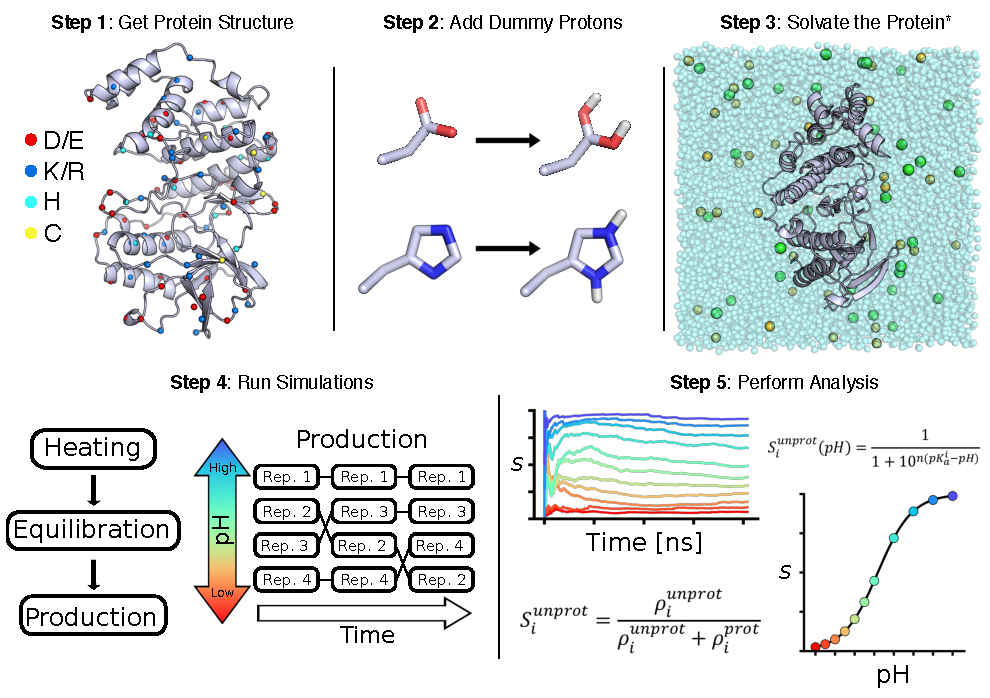
\includegraphics[width=6.6in]{figs/workflow_scheme.pdf}
    \caption{\textbf{Generalized CpHMD workflow} 
    *Mock Figure*  
    }
    \label{fig:intro}
\end{figure*}
 %--------------------------------------------- 

\subsection{Hybrid-Solvent CpHMD in CHARMM} % - Jack

Here, the steps and processes involved in running CpHMD simulations in CHARMM are presented. 
In the first part of each section (System Preparation, Equilibration, and Production) an example of how to run CpHMD on the small soluble protein BBL (PDBid: 1w4h)\cite{Ferguson_JMolBiol_2005_v353_p427} is used as an example case. 
To follow along the please download the CpHMD tutorial from our \href{https://gitlab.com/shenlab-amber-cphmd/cphmd-tutorial/-/tree/main/pH-REX_CpHMD_BBL_tutorial_in_CHARMM}{GitLab page}.
In the second part of the system preparation and equilibration section, supplemental information is provided discussing how to setup and run CpHMD simulation on transmembrane proteins.
Example input files for select portions of this process can be found from our \href{https://gitlab.com/shenlab-amber-cphmd/cphmd-tutorial/-/tree/main/MEMB_pH-REX_CpHMD_CHARMM_Examples}{GitLab page}.

\subsubsection{System Preparation}

% Figure Concept: Show image of the ASP in the double protonated (syn-Configuration) State

To begin one needs to obtain a protein structure from the \href{https://www.rcsb.org/}{Protein Data Bank} (PDB).\cite{Berman_NucleicAcidsRes_2000_v28_p235}
If there are any missing residues in the downloaded protein structure they need to be filled in.
I good tool for this is SWISS-MODEL\cite{Waterhouse_NucleicAcidsRes_2018_v46_p296}, which allows you to replace missing residues based on homology to like proteins.
In the first part of this section we will go through an example for preparing the small protein BBL (PDBid: 1w4h)\cite{Ferguson_JMolBiol_2005_v353_p427} and in the second part discuss the preparation of transmembrane proteins.

With the protein structure for BBL downloaded from PDB we clean the structure using the MMTSB\cite{Feig_JMolGraphModel_2004_v22_p377} tool \href{http://blue11.bch.msu.edu/mmtsb/convpdb.pl}{convpdb.pl}. 
Additionally, all histidine residue names need to be changed to HSP and this is done in one step with the following command. 
%
\begin{lstlisting}[language=bash]
$ perl convpdb.pl -out charmm22 -segnames
-renumber 1 1w4h.pdb | sed "s/HSD/HSP/g" 
> start.pdb
\end{lstlisting}
%
Here, the output is formatted for the CHARMM22 protein force fields (-out charmm22), the segment names are included in the output (-segnames), the resids are renumbered starting at 1, and the input file is "1w4h.pdb."
Changing all HSDs to HSPs allows for titration of both $\delta$ and $\epsilon$ protons later.
Although the resids have been renumbered starting from one this does not have to be the case. 
Next we add all the missing hydrogen atoms to the protein using the HBUILD facility\cite{Brunger_Proteins_1988_v4_p148} in CHARMM.
For ASP and GLU, dummy protons are placed in the $syn$ position, and the force fields contains a dihedral energy barrier (raised to 3 kcal/mol) to maintain them in this position, so they don't move to the less favorable and rarely sampled $anti$ position ("ghost" position).\cite{Khandogin_BiophysJ_2005_v89_p141, Mongan_JComputChem_2004_v25_p2038} 
Addition of the hydrogens requires two rounds of energy minimization: first, with 50 steps of steepest decent (SD), and second 10 steps of adopted basis Newton-Raphson (ABNR) with the a heavy atom harmonically restrained (50 kcal/mol) in both cases.
This will help remove any unfavorable hydrogen positions. 
In most cases the N- and C-terminus ends of the protein are truncated and require capping. 
For the N-terminus use the CH$_3$CO (patch ACE) and for the C-terminus use NH$_2$ (patch CT2) or NHCH$_3$ (patch CT3).
In special cases the free ionized form, NH$_{3}^{+}$ and COO$^+$, is used and can be set to be titratable when CpHMD is turned on. 
The input file "step1\_add\_h.inp" is an example of how to perform these steps on BBL and if CHARMM is installed can be run with the following command.
%
\begin{lstlisting}[language=bash]
$ charmm -i step1_add_h.inp -o step1.out
\end{lstlisting}
%
Additionally, the example script will check for disulfide bonds using a sulfur to sulfur atom distance of 2.5 \mbox{\AA}. 
After running any input file make sure to visualize the output to confirm all protonation states and additional features are correctly constructed. 
Now We move on to making a water box to solvate the system using a small box of pre-equilibrated TIP3P waters.
This is done by generating a plan of water boxes along the X- and Y-axis, then stacking planar water boxes along the Z-axis.
After that, the box is reshaped to a truncated octahedron. 
In the example script the water is placed such that $\sim$10$\mbox{\AA}$ of padding is between the protein and the edge of the periodic boundary condition.
Use the following command and input file to construct the water box.
%
\begin{lstlisting}[language=bash]
$ charmm -i step2_make_waterbox.inp -o step2.out
\end{lstlisting}
%
In the final step, the protein is solvated with the water box by placing the protein at the center of the box and removing all water molecules within 2.8 $\mbox{\AA}$ of the protein heavy atoms. 
This step involves several phases of minimization; first the protein heavy atoms are fixed and the system is minimized using both SB and ABNR for 50 steps each, then five stage of minimization are used with reducing harmonic restraints (100, 50, 25, 5, 0 kcal/mol) on the protein heavy atoms using 50 steps of SD and 100 steps of ABNR each stage. 
Run this step with the following command and input file.
%
\begin{lstlisting}[language=bash]
$ charmm -i step3_solvate.inp -o step3.out
\end{lstlisting}
%
With the system built you can now move on to the next step. 
Again, always remember to visualize the system and make sure everything has been constructed to your expectations. 

In some cases the protein crystal structure will include water molecular resolved in the PDB. 
This can be kept with a few modifications to the protocol above. 
First move all the water molecules into a separate PDB file and make sure the PDB file is properly formatted with the correct names, resnames, and has the correct column spacing.
Most error messages involving the handling of the crystal waters comes from the separate crystal water PDB not being properly formatted. 
You will need to make a new input file to add hydrogens to the water oxygen positions, like what was done with the protein and save the new water molecules as a CRD and PSF file. 
Now you will need to make another input file that reads in the protein coordinates and the crystal water coordinates and outputs a file with them merged together. 
The rest of the process now is similar to what was done above. 
You just need to make sure that in step3 solvate step the you don't accidentally delete these waters.

\noindent
\textbf{Transmembrane protein system preparation details}

Transmembrane proteins require a few additional steps to their preparation because they require a more rigorous equilibration. 
First we obtain the protein structure from the database \href{https://opm.phar.umich.edu/}{Orientations of Proteins in Membranes} (OPM). 
The OPM database orients the protein in the lipid bilayer using theoretical calculations with comparisons to experimental data, so an accurate placement of the protein in a lipid bilayer can be achieved.\cite{Lomize_Bioinformatics_2006_v22_p623}
Just like for soluble proteins any missing residues need to be added and then the missing hydrogens can be added.
Before the transmembrane protein system can be simulated with CpHMD, the lipid bilayer needs to be equilibrated using fixed charge MD simulations and this is done using any scalable MD engine like NAMD,\cite{Phillips_JComputChem_2005_v26_p1781} OpenMM,\cite{Eastman_PLoSComputBiol_2017_v13_pe1005659} or GROMACS.\cite{Abraham_SoftwareX_2015_v1-2_p19}
Thus, the protonation states of titratable groups need to be assigned based on any "Anticipated" pH condition described by wither experimental of physiological pH conditions. 
If there is not a pre-described pH condition the physiological pH (7.4) condition can be used giving the titratable residues the resulting charge states: Asp(-), Glu(-), Arg(+), Lys(+), Cys(0). 
Since His has a {\pka} near this pH condition special attention should be given to its protonation (singly or doubly protonated) and tautomeric state (HSD or HSE), based on any hydrogen bonding or salt-bridge interactions it can have. 
Like the soluble proteins the N- and C-terminus ends should be capped and if charged caps are used their protonation states should be considered and assigned. 
This is especially so for N-amino group since its solution {\pka} is 8.5,\cite{Nozaki_MethodsEnzymol_1967_v11_p715} only one pH unit above physiological pH.
Once hydrogens have been added and protonation states assigned, a short minimization is required to remove any poorly placed hydrogen positions.
Again, the system can be minimized in two round with 50 steps of SD followed by 10 steps of ABNR first with the heavy atoms either fixed or greatly harmonically restraint in the first round and with a reduced restraint in the second round.
With the protein prepared the rest of the system can be built and partially equilibrated to relax the systems structures (protein, lipids, ect.) following the CHARMM-GUI protocol for placing the lipids, solvating the system, and adding ions to achieve a solution salt concentration and to charge neutralize the system.\cite{Jo_PLoSONE_2007_v2_pe880}

\subsubsection{Equilibration}

\begin{checklist}{Equilibration Requirements}
\textbf{A list of files needed for the equilibration of a soluble protein}
\begin{itemize}
\item system PDB file 
\item system CRD file 
\item system PBC file
\item equilibration$\_$hphmd.inp
\end{itemize}
\end{checklist}

Equilibration of soluble protein systems for CpHMD is performed in several stages carried out at a single pH.
Since, CpHMD is turned on in the equilibration stages the residues allowed to titrate must be chosen, for this example Asp, Glu, and His are allowed to titrate, because of the pH range used during the production phase.
The pH chosen is normally the crystal pH condition of the PDB structure or a suitable pH for your system like physiological pH 7.4.
Before starting the simulations determine implicit solvent ionic strength (0.15 M in the example) and temperature (298 K in the example).
To use CpHMD in CHARMM add the following \href{https://hpc.nih.gov/apps/charmm/c42b2html/phmd.html}{PHMD module} to your input file after streaming in the GBSW parameters and reading the CpHMD parameters. 
%
\begin{lstlisting}
PHMD PAR 23 wri 25 PH 7.4 NPRI 500 PHFRQ 5 
    MASS 10.0 BARR 0.0 BETA 5.0 TEMP 300 LAM -
    sele resn ASP .or. resn GLU .or. resn HSP end
\end{lstlisting}
%
Here, PH sets the pH environment of the simulation, NPRI sets the frequency to print the lambda values, PHFRQ sets the update frequency of the lambda file, TEMP sets the temperature for the configuration of the titration coordinates and should be the same as the simulation temperature, MASS is the fictitious mass of the titration coordinate, BARR is the quadratic barrier height for each titration coordinate, BETA is the friction coefficient, and LAM tells the PHMD module to output lambda values.
The last line in the module states which residues should be allowed to titrate. 
The length of each stage depends on the system and should be adjusted accordingly, stages lasting 40 to 120 ps have been used by group for previous projects.
For the BBL example all heating/equilibration stages were run for 20 ps, since the system is small and stable. 
Firstly the system is heated, here we use an NVT ensemble and set and initial temperature to what was used to resolve the either the X-ray crystal or the cryo-EM structure. 
If the system does not require heating the initial and final temperatures can be set to be the same value and the system can equilibrate the water positions under the NVT ensemble.
Next we run a series of NPT ensemble equilibration stages with diminishing harmonic constraint on the heavy atom positions. 
The idea here is to slowly relax the system removing any high energy interactions and to allow for the initialization protonation states.
Using four equilibration stages the harmonic constraints on the protein heavy atoms are reduced with the following values 5.0, 1.0, 0.1 (kcal/mol), and then in the last stage all harmonic restraints are released.
After each equilibration make sure the energies of the system have equilibrated.
You are now ready to start the production run. 
The example equilibration input provided moves through each heating/equilibration stage in one input file (equilibration$\_$hphmd.inp). 

\noindent
\textbf{Transmembrane protein system preparation details}

The equilibration of transmembrane proteins is a little more involved than soluble proteins, because of the equilibration of the lipid membrane. 
The transmembrane protein system has now undergone an initial relaxation according to the CHARMM-GUI protocol, and as mentioned in the system preparation fixed charge simulations need to be conducted to equilibrate the lipid bilayer.
Here, the protein heavy atoms are harmonically restrained using a 1.0 kcal/mol/$\mbox{\AA}^2$ until the lipid bilayer is equilibrating. 
Initially, the simulation is briefly simulated with a 0.2 ns NVT ensemble simulation.
Then the a much longer NPT ensemble simulation is run to fully equilibrate the simulation. 
These simulations should be run until the surface area per lipid, bilayer thickness, and lipid order parameters are near or within error limits of experimental lipid composition you are simulating.\cite{Huang_Shen_2020_}
These three lipid bilayer metrics are frequently used to assess the phase behaviour and fine structure of the simulated bilayer.\cite{Klauda_JPhysChemB_2010_v114_p7830}
Simulations up to 100 ns can be necessary for proper equilibration of the lipid bilayer.

Following equilibration of the lipid bilayer the system can now be equilibrated at a single pH with CpHMD. 
To start this processes, the dummy protons need to be added back on to the all Asp, Glu, and His side chains. 
This can be done in the exact same way as it was done in the system preparation of soluble proteins and should also be minimized in a similar way.
Now three short equilibrations can be run using CpHMD at a single pH, example inputs for these three equilibration are provided on our GitLab site [Add GitLab Information]. 
Like a soluble protein the pH used should be the crystal pH, physiological pH, or a experimentally relevant pH.
The first two simulations are performed with the protein harmonically restrained (1.0 kcal/mol/$\mbox{\AA}^2$) for 0.1 ns, but the first simulation uses the NVT ensemble and the second uses the NPT ensemble.
The third simulations continues with an NPT ensemble for 0.8 ns with all restraints removed. 
For membrane-enable CpHMD simulations the tmemb features needs to be added to the \href{https://hpc.nih.gov/apps/charmm/c42b2html/gbsw.html}{GBSW module} in the CHARMM input file. 
%
\begin{lstlisting}
gbsw hybrid sgamma 0.0 nang 50 conc 0.15 temp 310 
     tmemb 30 msw 2.5 rcyln 15                      
     sele SOLU end
\end{lstlisting}
%
Here, sgamma is the non-polar surface tension coefficient, nang is the number of angular integration points, and conc is the salt concentration.
The inputs variables tmemb, msw, and rcyln are used to build a low dielectric slab to represent the lipid bilayer in the GBSW model with a high dielectric hole centered around the protein.
The tmemb variable sets the slab thickness ($\mbox{\AA}$) and should be set to the average difference in the $Z$ positions of the lipid C2 atoms from the top and bottom leaflets, this will vary for different lipid types. 
The msw variable is the half membrane switching length\cite{Im_BiophysJ_2003_v85_p2900} for the dielectric transition region between the low-dielectric slab and the bulk solution, and is commonly set to 2.5 $\mbox{\AA}$.
Finally, rcyln is the radius of the high dielectric hole in the low dielectric slab and should set so there is minimal overlap between the protein and lipids.
The protein selection, the last line on in the GBSW module, required the protein selection to place the hole at the center of the protein.
Without restraints on the protein heavy atoms, a cylindrical restraint with a harmonic force constant (0.1 kcal/mol/$mbox{\AA}$) needs to be applied to the protein to prevent lateral drift of the protein. 
This can be done using the MMFP facility in CHARMM.

\subsubsection{Production}

\begin{checklist}{Production Run Requirements}
\textbf{A list of files needed for the production run of a soluble protein}
\begin{itemize}
\item system PSF file
\item system CRD file 
\item system PBC file
\item final equilibration RST file
\item production$\_$hphrex.inp
\item rep.cmd
\end{itemize}
\end{checklist}

The CpHMD production stage is the same for both soluble and transmembrane proteins. 
The only differences are in the set up of the GBSW module to include a low dielectric slab to represent the lipid bilayer for transmembrane simulations, which is discussed in the equilibration stage. 
To begin the production run one must chose a pH range to simulation over and how many 
pH replicas to use. 
For instance, a protein of interest may be active over a particular pH range or you might want to capture conformational dynamics that include specific titratable residues such as Asp or His. 
Next you need to decide how many pH replicas to use for your production run. 
Somethings to consider are how many CPUs you have available and how many CPUs you want to allocate to each replica. 
Simulations with CHARMM do not scale well past 8 CPUs, so for a job using 16 replicas you will need 128 CPUs. 
The spacing of the pH replicas needs to be close enough to obtain sufficient exchange probabilities (e.g., 20$\%$).
Typically, to obtain overlap between potential energy distribution of neighboring replicas a pH spacing in increments of 0.25 or 0.5 is required. 
Exchange attempts are made every 500 to 1000 steps, and a typical CpHMD simulation of this type will have an average exchange rate of $\sim$40$\%$, if exchange rates are too low more replicas can be added to fill in the spacing between replicas.
To achieve enhanced sampling several replicas show move across all pH replicas.
To use pH-based replica exchange in CHARMM the following \href{https://hpc.nih.gov/apps/charmm/c39b2html/repdstr.html}{REPD} module must be used.
%
\begin{lstlisting}
REPD NREP 8 PHMD EXLM FREQ 1000 UNIT 17
\end{lstlisting}
%
Here, the REPD command initiates replica exchange, NREP states the number of replicas to use, in this case 8, and PHMD states this is pH-based replica exchange and allows for the exchange of $\lambda$ along with the spatial coordinates.
Next, EXLM allows for Hamiltonian exchange and FREQ is how often an exchange is attempted. 
Then to run several replicas in parallel CHARMM reads in a rep.cmd file for each pH replica with the syntax, rep.cmd$\_$0, rep.cmd$\_$1, to rep.cmd$\_$(NREPS), using the following command in the input file.
%
\begin{lstlisting}
stream rep.cmd
\end{lstlisting}
% 
Notice this command lacks the '$\_0$' portion of the name.
In each of the rep.cmd file you will have the command that states the pH environment of the at replica.
%
\begin{lstlisting}
PHMD RESPH OLDPH @crysph NEWPH @ph PKATEMP @temp
\end{lstlisting}
%
Where OLDPH is the pH used in the equilibration and NEWPH is the pH of the replica.
finally, PKATEMP should be set to the same temperature of the simulation. 
The rest of the replica exchange set up follows a standard molecular dynamics run in CHARMM.
Production run inputs for BBL (production$\_$hphrex.inp and rep.cmd) can be used to run one 2 ns stage of pH-Replica Exchange CpHMD.


\subsubsection{General MD and CpHMD Settings}
% CHARMM Specific
% Things to Include: 
%   -) FFs
%   -) Thermostats
%   -) Baristas
%   -) Cutoffs
%   -) ect...

For all simulations with CHARMM the protein is represented with CHARMM22/CMAP force fields.\cite{MacKerell_JPhysChemB_1998_v102_p3586,MacKerell_JComputChem_2004_v25_p1400}
For the solvent the CHARMM modified TIP3P water model are used and for any ions or lipid molecules that might be included the CHARMM36 force fields are used.\cite{Klauda_JPhysChemB_2010_v114_p7830}
To be consistent with the CHARMM36 development protocol all van der Waals energies are calculated with a switching function from 10 to 12 $\mbox{\AA}$ with a cutoff at 14 $mbox{\AA}$. 
All simulations are conducted under periodic boundary conditions. 
The PME method\cite{Darden_JChemPhys_1993_v98_p10089} is used to calculate the long-range electrostatic energies and forces with a real space calculation cutoff of 12 $\mbox{\AA}$, 1 $\mbox{\AA}$ grid spacing, and a 6th-order spline interpolation. 
In CHARMM the non-bond neighbor list is updated heuristically. 
Additionally, the SHAKE\cite{Ryckaert_JComputPhys_1977_v23_p327} algorithm in CHARMM is used to constrain all bonds involving hydrogens to allow for a 2 fs time step. 
For NPT simulations the temperature is maintained with the N\'{o}se-Hoover thermostat.\cite{Nose_MolPhys_1984_v52_p255, Hoover_PhysRevA_1985_v31_p1695}
The pressure is maintained with the CHARMM implemented Langevin piston pressure-coupling algorithm.\cite{Feller_JChemPhys_1995_v103_p4613}

For CpHMD simulations, the default GBSW radii\cite{Nina_JPhysChemB_1997_v101_p5239, Chen_JAmChemSoc_2006_v128_p3728} are used for the proteins and any small molecules the generic atomic radii in the GBSW radii file or van der Waals radii in the force field\cite{Knight_JComputChem_2011_v32_p2909} should be used. 
As shown in the example inputs the titration ($\lambda$) and tautomer ($\chi$) should be updated every 5 MD steps, allowing for water and lipid relaxation.\cite{Wallace_JChemTheoryComput_2011_v7_p2617}
A friction coefficient of 5 ps$^{-1}$ should be used for Langevin dynamics and the mass of the titration coordinate ($\lambda$ and $\chi$) should be 10 atomic mass units. 

\subsection{All-atom PME CpHMD in CHARMM} % - Yandong

Minor modification of the workflow for 
hybrid-solvent CpHMD above is needed 
to setup and run an all-atom PME CpHMD 
simulation in CHARMM. 

To maintain a constant net charge during 
all-atom PME CpHMD simulations, 
titratable water molecules  
or coions should be added to the 
system as built above \cite{Wallace_Shen_2012_J.Chem.Phys.}.
In specific, each acidic (ASP or GLU) or 
basic residue (HSP or LYS) is 
coupled with one coion that can convert 
to a hydroxide (TIPU) or hydronium (TIPP) 
\cite{Chen_Shen_2013_Biophys.J.}. 
Together with the salt ions, the coions 
can be placed in the water box with 
the input script step3\_add\_ions.inp.
Likewise, water molecules within 2.8 \AA\ 
of ions and the protein are removed 
with the script step4\_solvate.inp. 

To run an all-atom PME CpHMD simulation, 
the GBSW module should be 
removed first such that PME module is 
utilized in either conformational or 
titration dynamics \cite{Huang_Shen_2016_J.Chem.TheoryComput.}. 
Second, the coupling information should 
be specified. 
As to BBL that 
contains 3 ASP, 3 GLU and 2 HSP, below 
are the parameters required when PHMD module 
is invoked.  

%
\begin{lstlisting}
PHMD PAR 23 wri 25 PH 7.0 NPRI 500 PHFRQ 5 
    MASS 10.0 BETA 5.0 TEMP 300 LAM -
    sele resn ASP .or. resn GLU .or. TIPU .or. 
    resn HSP .or. TIPP end - 
    qcouple 8 - 
    resi 4  resc 4789 -
    resi 16 resc 4790 -
    resi 20 resc 4791 -
    resi 36 resc 4792 -
    resi 37 resc 4793 -
    resi 39 resc 4794 -
    resi 17 resc 4771 -
    resi 41 resc 4772 
\end{lstlisting}
%
Here TIPU and TIPP are selected as titratable too. 
The parameter qcouple, 8 in this case, indicates 
the count of coupled pairs listed behind. 
The second and forth 
colunms correspond to the indices of 
titratable residues and the coions 
associated respectively.

Finally, the calculated \pka's are 
corrected with the following formula 
to account for the finite-size error 
\cite{Huang_Shen_2016_J.Chem.TheoryComput.}.

\begin{eqnarray}
\label{eq:pka_corr}
\Delta\Delta{G}^{\rm offset} &=&
\frac{2 \pi}{3} \kappa \gamma^{\rm solv} Q 
\left(\frac{N}{V}
- \rho^{\rm pure} \right) \\
\Delta pK_a^{\rm corr} &=& \pm \frac{\Delta\Delta{G}^{\rm offset}}{ln(10)RT},
\end{eqnarray}
where $\gamma^{\rm solv}$ is 0.764 e$\cdot$ {\AA$^2$} 
for TIP3P water model. 
$\kappa$ is the electrostatic constant, 
which is 332.0 kcal 
$\cdot$ {\AA} $\cdot$ mol$^{-1}$e$^{-2}$. 
The solvent number density $\rho^{\rm pure}$ is 
0.0333679 {\AA}$^3$ for water at ambient temperature 
and pressure. 
Q is -1 for acidic groups and +1 for basic groups. 
The negative sign is for acid groups and positive sign 
is for basic groups.
Thus, $\Delta$\pka$^{\rm corr}$ is negative for both 
acidic and basic groups. 
N is the number of solvent and V is the volume of the box 
measured at equilibrium, which can be approximated 
with the initial volume $V^{\rm init}$ times 0.93. $V^{\rm est} = L^3$ for a cubic box and $V^{\rm est} = 0.77L^3$ for a truncated octahedron box, where L denotes the cubic 
box size. R is the Boltzmann constant and T is the temperature.

\subsection{Implicit-Solvent CpHMD in AMBER} % - Ruibin
\subsubsection{System Preparation}
To prepare a protein system in implicit solvent for CpHMD in Amber, the process is similar to the hybrid-solvent CpHMD in CHARMM but much simpler. We have a \href{https://gitlab.com/shenlab-amber-cphmd/cphmd-prep}{cphmd-prep} package (and soon a web server) to prepare the Amber GBNeck2-CpHMD inputs and instructions to run related CpHMD simulations by one line bash command via the 'CpHMD\_Prepare.sh' script. The script accepts either a PDB ID (-p|--pdbid flag) whose PDB file is downloadable from RCSB to the working machine or a user-prepared PDB file (-f|--pdbfile flag) stored in the machine. After that, PDBFixer (powered by OpenMM) is used to extract the desired chain (-c|--chainid flag) and model (-m|--modelid) protein structure only and remove all other parts like ions, ligands, waters, or unwanted chains. Missing heavy atoms and residues are then added by PDBFixer. Importantly, capping ligands ACE and NH$_2$ are added to cap the N and C terminus to suppress unwanted electrostatic effects from otherwise charged terminus. After the PDB file is prepared, tleap in Amber (or Ambertools) is used to build hydrogen and dummy hydrogen atoms according to the titratable types (-type|--residuetypes flag) set by the user. Specifically, the user can choose one or a combination in 'Asp Glu His Cys Lys'. After the system is prepared, it is required by GBNeck2-CpHMD that the GB radii of His HD1 and HE2, Cys SG, Asp OD1 and OD2, and Glu OE1 and OE2 atoms should be changed to 1.17, 2.00, 1.40, and 1.40 {\AA} respectively; and the interactions between the two dummy hydrogens in Asp and Glu should be excluded in the non-bonded interaction terms. This is automatically done in `CpHMD\_Prepare.sh` too. 

Even though our cphmd-prep tool can prepare a system for most cases, the user with different needs can use other tools to do the same or different tasks as instructed by cphmd-prep. Nevertheless, here we show two simple examples of how to use 'CpHMD\_Prepare.sh' to prepare a GBNeck2-CpHMD simulation system. The first is an EFGR kinase with provided PDB ID 5U8L and we want to know the protonation states and possible {\pka's} of His, Cys, and Lys near the psychological pH condition 7.4. 
%
\begin{lstlisting}
CpHMD_Prepare.sh -p 5U8L -m A -pmin 5.5
                 -pmax 9.5 -type 'His Cys Lys'
\end{lstlisting}
%
Note that we omit chain ID(s) because 5U8L only has one chain whose chain ID is A but we do specify the model ID as A because there are two alternative model IDs for 5U8L, A and B. We choose the pH range from 5.5 to 9.5 with a default interval 0.5 units, which covers about 2 pH units from the two directions of 7.4, making the total number of independent pH calculations to be 9. The other important settings are the simulation length, temperature and implicit ionic strength, which are 20 ns, 300 K, and 150 mM by default. Four important files will be generated if the command runs successfully. The 5U8L\_ModelA\_A\_fixed.rst7 file is an Amber topology rst7 file with initial coordinates; the cphmd\_5U8L\_ModelA\_A\_fixed.parm7 file is an Amber parameter parm7 file; the 5U8L\_ModelA\_A\_fixed\_phmdin file is an GBNeck2-CpHMD job control input file; the gbneck2\_input.parm file is the GBNeck2-CpHMD parameter file which is the same for all GBNeck2-CpHMD calculations. Other files including Amber input files are also generated and they will be explained later.

The second example is to quickly estimate the {\pka's} of all Asp, Glu, His, Cys, and Lys residues in SNase with a PDB file 3BDC.pdb. The command is
%
\begin{lstlisting}
CpHMD_Prepare.sh -f 3BDC.pdb -m A -pmin 1.0 
                 -pmax 12.0 -l 4
\end{lstlisting}
%
Here we feed the script with the PDB filename and use a much larger pH range from 1.0 to 12.0 so that the Asp, with a model {\pka} of 3.7, and Lys, with a model {\pka} of 10.4, residue types can both titrate in the pH range. In addition, we use a much shorter length, 4 ns, because we only want a rough estimation of the {\pka's}. We omit the -type flag because the all five residue types are included by default. Similar files as the previous example will be generated. The user may notice that many more Amber input files are generated. They differ in the solveph keyword that is required to perform CpHMD calculations in different pH conditions.

System minimization with constraints on heavy atoms (except for two terminal and capping residues whose all atoms are allowed to move) is performed after preparing the aforementioned Amber input files. The constraint strength is 50 kcal/mol/\AA$^2$. The input file has a name end with *\_fixed\_mini.mdin which can be found in the generated files. The minimization last 1000 steps with the first 500 steps for steepest descent algorithm and the remaining 500 steps for conjugate gradient steps. After minimization, a *\_mini.rst7 is obtained for the next step. For convenience, all commands for minimization, equilibration, and production runs are listed in the README file generated by the 'CpHMD\_Prepare.sh' file, same for the below steps.

\subsubsection{Equilibration}
For implicit solvent based CpHMD, heating is very fast and thus not required. We do have four short steps of equilibration that the constraintes on heavy atoms are gradually released from 5.0, 2.0, 1.0, to 0.0 kcal/mol/\AA$^2$. Each step last 2000 steps or 4 ps and the total length is 16 ps. In equilibration and production steps, CpHMD is turned on by setting the iphmd keyword to 1 for GBNeck2-CpHMD.

\subsubsection{Production}
For production runs, we can either use CPU pH replica exchange (pHREX), GPU independent pH (pHInd), or GPU asynchronous pH replica exchange styles (\href{https://gitlab.com/shenlab-amber-cphmd/async_ph_replica_exchange}{Async-pHREX}). Replica exchange simulations usually need shorter time for convergence in {\pka} predictions but GPU acceleration can overcome the simulation time problem, and thus Async-pHREX is recommended over the other two styles. Although the asynchronous replica exchange we implemented is in the script level, it still combine the significantly good parts of GPU acceleration and replica exchange enhanced sampling, especially for large systems or the GPUs are the old models. We run pHREX just like we run other replica exchange simulations in Amber, i.e., we need a group file which contains the command line flags and inputs for every pH condition and then run with mpirun. For pHInd, we run each pH condition independently on different GPUs in the same machine by changing the CUDA\_VISIBLE\_DEVICES environment variable or even on GPUs in different machines. For Async-pHREX, we have to use a template input file from which temporary input files for different pH conditions at a replica exchange attempt can be generated. Output files are concatenated according to pH conditions instead of replicas in the pHREX method. For all these three methods, we can use the -rex flag to control which method is going to be used and the related commands can be found in the README file as well.
% Here we can describe a few different styles of production run with CpHMD. 
% this section can be broken down into three sections
%   1.) Single-pH runs with CpHMD Simulations in AMBER
%   2.) Async-pHREX with CpHMD simulations in AMBER

\subsubsection{MD Specific Settings}
For best performance regarding {\pka} prediction speed and accuracy, there are several settings that we think should be fixed in Amber GBNeck2-CpHMD. GBNeck2 implicit solvent model works best with the Amber FF14 force field. Langevin thermostat with a collision frequency 1 ps$-1$ is used to maintain system temperature. Non-bonded cutoff is 999.9 \AA which means not cutoff is used practically. CpHMD specific lambda files are usually saved every 1000 MD steps while trajectory files are saved every 10000 steps to save I/O time. 
% Amber Specific
% Things to Include: 
%   -) FFs
%   -) Thermostats
%   -) Baristas
%   -) Cutoffs
%   -) ect...

\section{Lambda File Analysis} % - Jack / Vini

The lambda file outputs provide us the propagation of $\lambda$ (titration state) and $x$ (tautomeric state) coordinates from titratable residues along the CpHMD simulation. Such information allows us to calculate the protonation state changes during the dynamics, the pKa value of each ionizable residue and also monitoring the pKa convergence. In order to facilitated these analysis, our research group developed a Python tool (cphmdanalysis.py) that possesses several classes to run calculations in lambda files and log files, and can be found at GitLab: \href{https://gitlab.com/shenlab-amber-cphmd/cphmd-analysis}{CpHMD-Analysis}. This tool can also plot the unprotonation fraction and pKa of selected titratable residues.

From each simulated pH, we can calculate the population of the $i$th titratable residue in the protonated state ($N_i^{\rm Prot}$, $\lambda_i < 0.1$) and in the unprotonated state ($N_i^{\rm Unprot}$, $\lambda_i > 0.9$). Thus, we can obtain the unprotonated fraction of this residue, 

\begin{equation}
S_i = \frac{N_i^{\rm Unprot}}{N_i^{\rm Prot} + N_i^{\rm Unprot}}.
\end{equation}

The convergence of the $S_i$ values during the CpHMD steps indicates that the simulation reached a protonation state sampling equilibrium.    

Finally, we can fit the calculated $S_i$ at several pHs using the generalized form of the Henderson-Hasselbach equation,

\begin{equation}
S_i = \frac{1}{1+10^{n(\rm pK_{a,i} - pH)}},
\end{equation}
where $n$ is the Hill coefficient, and indicates the degree of cooperativity between the titratable groups. 


% Here we can describe how to analyze CpHMD results
%   1.) Calculations of Unprot. Fractions
%   2.) Calculations pKa  
%   3.) How to Monitor pKa Convergence
%   3.) Additional Analysis could include proton-coupling, ect... 

% Figure Concept: Here we should have a 2 panel figure. 
%   -) Panel 1: Raw Lambda Value versus time @ a single pH with a duel y-Axis and over the plot we showing the running S-value. 
%   -) Panel 2: We show a titration Curve

\section{Parameterization} % - Jack/Ruibin
To perform CpHMD simulations on a new titratable residue, accurate values for the parameters of $U^{model}$ are required. The basic method for obtaining these parameters is to simulate a model compound containing an analog of the residue in question at several fixed values of $\theta_{i}$ and $\theta^{x}_{i}$ with $U^{barr}$ and $U^{pH}$ set to 0, compute the derivatives of the free energy with respect to $\theta_{i}$ and $\theta^{x}_{i}$, and fit those derivatives to eq. \ref{eq:Umod_1d} and \ref{eq:double}.

Note that these fittings should be performed on the $\theta$ and $\theta_{x}$ variables directly rather than on $\lambda$ and $x$ because the nonlinearity in the definitions of $\lambda$ and $x$ cause difficulties in the fitting.

Typically we are interested in three different kinds of titratable residues in most proteins, residues, such as Lys, that have a single titratable site, residues, such as Glu and Asp, that have two titratable sites with identical microspcopic pKa's, and residues, such as His, that have two titration sites with different microscopic pKa's. Each of these cases have different forms for their $U^{model}$ and therefore require somewhat different methods.

First, for residues like Lys with a single titratable site, we only need to consider a single titration variable, $\theta$. For these residues we construct a model compound for which the experimental pKa is known, such as the blocked amino acid, and run simulations with fixed values of $\theta$ and fit the resulting $\partial U/\partial\theta$ to eq. \ref{eq:Umod_1d}.

Second, for residues, like His, that contain two nonidentical intertacting titratable sites, eq. \ref{eq:double} can be written as

\begin{align}
U^{model}= & A_{10}\lambda^{2}x^{2}+2\left(A_{1}B_{1}-A_{0}B_{0}\right)\lambda x+\nonumber \\ & 2\left(A_{0}B_{0}-A_{1}B_{1}-A_{10}B_{10}\right)\lambda^{2}x+ \nonumber \\ & A_{1}\lambda^{2}-2A_{1}B_{1}\lambda\label{eq:his}
\end{align}

The six parameters $A_{0}$, $A_{1}$, $B_{0}$, $B_{1}$, $A_{10}$, and $B_{10}$ can be obtained by running simulations on the model compound at different values of $\theta$ and $\theta_{x}$ with $U^{model}$, $U^{barr}$, and $U^{pH}$ set to 0, computing the derivatives of the free energy with respect to $\theta_{i}$ and $\theta^{x}_{i}$, and fitting those derivatives to this equation. Note once again that although eq. \ref{eq:his} is written in terms of $\lambda$ and $x$ for clarity, the fitting should be performed against $\theta$ and $\theta_{x}$ to avoid issues arising from nonlinearities near the endpoints.

Finally, for residues like Asp and Glu, that contain two identical interacting titratable sites, eq. \ref{eq:double} reduces to

\begin{align}
    U^{model}= & \left(R_{1}\lambda^{2}+R_{2}\lambda+R_{3}\right)\left(x-R_{4}\right)^{2}+\left(R_{5}-R_{1}R_{4}^{2}\right)\lambda^{2} \nonumber\\ & -\left(2R_{5}R_{6}+R_{2}R_{4}^{2}\right)\lambda \label{eq:asp}
\end{align}

As before, the six parameters $R_{1}$ to $R_{6}$ can be obtained by running simulations on the model compound at different values of $\theta$ and $\theta_{x}$ with $U^{model}$, $U^{barr}$, and $U^{pH}$ set to 0, computing the derivatives of the free energy with respect to $\theta$ and $\theta^{x}$, and fit those derivatives to this equation. Note once again that although eq. \ref{eq:asp} is written in terms of $\lambda$ and $x$ for clarity, the fitting should be performed against $\theta$ and $\theta_{x}$ to avoid issues arising from nonlinearities near the endpoints.

\subsection{Parameterization settings and fitting procedure}
As discussed above, the key step to parameterizing a new residue is to run simulations with fixed values of $\theta$ and $x$ with $U^{barr}$, $U^{model}$, and $U^{pH}$ set to 0. This can be accomplished in Amber by setting the options prlam to false, prderiv to true, and phtest to true in the phmdin file and setting ph{\_}theta to the desired values of $\theta$ and $x$ and vph{\_}theta to 0 in the phmdstrt file.

As discussed above, the procedure for parameterizing a residue, such as Lys, with a single titratable site is pretty straightforward, just run at several values of $\theta$ (We generally find that $\theta=\left(0.0,0.2,0.4,0.6,0.785,1.0,1.2,1.4,1.5708\right)$ work well). In contrast, parameterizing two site residues is more complicated because the energy surface is two-dimensional. What follows is therefore a description of the method we usually use to parameterize these residues, although other approaches are possible.

First, for residues, such as His, with two titration sites with different microscopic pKa's, we generally run simulations at $\theta_{x}=0$ and $\theta=\left(0.0,0.2,0.4,0.6,0.785,1.0,1.2,1.4,1.5708\right)$. The parameters $A_{0}$ and $B_{0}$ can then be computed by fitting $\partial U/\partial\theta$ to

\begin{equation}
    \frac{\partial U}{\partial\theta}=2A_{0}\sin\left(2\theta\right)\left(\sin^{2}\left(\theta\right)-B_{0}\right).
\end{equation}
Next, the parameters $A_{1}$ and $B_{1}$ can be computed by running simulations at $\theta_{x}=1.5708$ and $\theta=\left(0.0,0.2,0.4,0.6,0.785,1.0,1.2,1.4,1.5708\right)$ and fitting $\partial U/\partial\theta$ to

\begin{equation}
    \frac{\partial U}{\partial\theta}=2A_{1}\sin\left(2\theta\right)\left(\sin^{2}\left(\theta\right)-B_{1}\right).
\end{equation}
Finally, $A_{10}$ and $B_{10}$ can be computed by running simulations at $\theta=1.5708$ and $\theta_{x}=\left(0.0,0.2,0.4,0.6,0.785,1.0,1.2,1.4,1.5708\right)$ and fitting $\partial U/\partial\theta_{x}$ to

\begin{equation}
    \frac{\partial U}{\partial\theta_{x}}=2A_{10}\sin\left(2\theta_{x}\right)\left(\sin^{2}\left(\theta_{x}\right)-B_{10}\right).
\end{equation}

Finally, for residues, such as Asp, that have two identical interacting titrating sites we have to find parameters $R_{1}$ to $R_{6}$. To start with, we generally run simulations at combinations of $\theta=\left(0.0,0.2,0.4,0.6,0.785,1.0,1.2,1.4\right)$ and  $\theta_{x}=\left(0.0,0.2,0.4,0.6,0.785,1.0,1.2,1.4,1.5708\right)$, compute $A\left(\theta\right)$ and $B\left(\theta\right)$ at each value of $\theta$ by fitting $\partial U/\partial\theta_{x}$ to

\begin{equation}
    \frac{\partial U}{\partial\theta_{x}}=2A\left(\theta\right)\sin\left(2\theta_{x}\right)\left(\sin^{2}\left(\theta_{x}\right)-B\left(\theta\right)\right),
\end{equation}
compute $A\left(\theta_{x}\right)$ and $B\left(\theta_{x}\right)$ at each value of $\theta_{x}$ by fitting $\partial U/\partial\theta_{x}$ to

\begin{equation}
    \frac{\partial U}{\partial\theta}=2A\left(\theta_{x}\right)\sin\left(2\theta\right)\left(\sin^{2}\left(\theta\right)-B\left(\theta_{x}\right)\right),
\end{equation}
obtain estimates of $R_{1}$, $R_{2}$, and $R_{3}$ by fitting $A\left(\theta\right)$ to

\begin{equation}
    A\left(\theta\right) = R_{1}\sin^{4}\left(\theta\right)+R_{2}\sin^{2}\left(\theta\right)+R_{3},
\end{equation}
setting $R_{4}=0.5$ (guaranteed because the two titrating sites are identical), obtain an estimate of $R_{5}$ by fitting $A\left(\theta_{x}\right)$ to

\begin{equation}
    A\left(\theta_{x}\right)=a_{0}\sin^{4}\left(\theta_{x}\right)+a_{1}\sin^{2}(\theta_{x})+R_{5},
\end{equation}
and finally obtain an estimate of $R_{6}$ by fitting $B\left(\theta_{x}\right)$ to

\begin{equation}
    B\left(\theta_{x}\right)=a_{0}\sin^{4}\left(\theta_{x}\right)+a_{1}\sin^{2}(\theta_{x})+R_{6},
\end{equation}
% Here is a single-column checklist that consists of multiple sub-checklists
\begin{Checklists}

\begin{checklist}{A list}
\textbf{Single-column checklists are also straightforward by removing the asterisk}
\begin{itemize}
\item First thing let's do an item which breaks across lines to see how that looks
\item Also remember
\item And finally
\end{itemize}
\end{checklist}

\begin{checklist}{Another list}
\textbf{This is some further description.}
\begin{itemize}
\item First thing
\item Also remember
\item And finally
\end{itemize}
\end{checklist}

\end{Checklists}



\section{Author Contributions}
%%%%%%%%%%%%%%%%
% This section mustt describe the actual contributions of
% author. Since this is an electronic-only journal, there is
% no length limit when you describe the authors' contributions,
% so we recommend describing what they actually did rather than
% simply categorizing them in a small number of
% predefined roles as might be done in other journals.
%
% See the policies ``Policies on Authorship'' section of https://livecoms.github.io
% for more information on deciding on authorship and author order.
%%%%%%%%%%%%%%%%

(Explain the contributions of the different authors here)

% We suggest you preserve this comment:
For a more detailed description of author contributions,
see the GitHub issue tracking and changelog at \githubrepository.

\section{Other Contributions}
%%%%%%%%%%%%%%%
% You should include all people who have filed issues that were
% accepted into the paper, or that upon discussion altered what was in the paper.
% Multiple significant contributions might mean that the contributor
% should be moved to authorship at the discretion of the a
%
% See the policies ``Policies on Authorship'' section of https://livecoms.github.io for
% more information on deciding on authorship and author order.
%%%%%%%%%%%%%%%

(Explain the contributions of any non-author contributors here)
% We suggest you preserve this comment:
For a more detailed description of contributions from the community and others, see the GitHub issue tracking and changelog at \githubrepository.

\section{Potentially Conflicting Interests}
%%%%%%%
%Declare any potentially competing interests, financial or otherwise
%%%%%%%

Declare any potentially conflicting interests here, whether or not they pose an actual conflict in your view.

\section{Funding Information}
%%%%%%%
% Authors should acknowledge funding sources here. Reference specific grants.
%%%%%%%
We acknowledge financial support from the National Institutes of Health (R01GM098818 and R01CA256557).

\section*{Author Information}
\makeorcid

\bibliography{Bib/JanaShenLab.bib}

%%%%%%%%%%%%%%%%%%%%%%%%%%%%%%%%%%%%%%%%%%%%%%%%%%%%%%%%%%%%
%%% APPENDICES
%%%%%%%%%%%%%%%%%%%%%%%%%%%%%%%%%%%%%%%%%%%%%%%%%%%%%%%%%%%%

%\appendix


\end{document}
